% TempO — ICLR submission draft. Swap \documentclass + iclr style file when the
% ICLR 2027 kit is released; prose is style-agnostic.
\documentclass[10pt]{article}
\usepackage[margin=1in]{geometry}
\usepackage{booktabs,amsmath,graphicx,url,xcolor}
\usepackage[numbers]{natbib}
\newcommand{\todo}[1]{\textcolor{red}{[TODO: #1]}}
\newcommand{\tempo}{\textsc{Tempo}}

\title{Temporal Observability for Coding Agents}
\author{Anonymous}
\date{}

\begin{document}
\maketitle

\begin{abstract}
Coding agents are correctness-supervised but time-blind: the harness reports
whether a command succeeded, never how long it took. As a result, agents cannot
notice that their own edit--build--test loop is slowing down --- they re-run
90-second test suites after one-line edits, block on waits they sized by
guesswork, and rebuild environments they already built. We call the resulting
degradation \emph{loop rot}. We first quantify the problem with a measurement
study of 500 public Terminal-Bench~2.0 leaderboard trajectories across 10
agent--model combinations: temporal waste is a long-tail phenomenon (median
3.7\% of wall-clock, 90th percentile 34\%), roughly 8\% of task failures are
time-management deaths, and a same-model/two-harness natural experiment shows
the harness's temporal interface alone shifts median waste from 0.1\% to 7.2\%.
We then present \tempo{}, a harness-level mechanism that makes iteration cost
observable --- injecting per-command elapsed time, cumulative budget state, and
slow-command trend signals into the agent's observation space --- and
\textsc{RotBench}, a benchmark of growth-driven developability-decay tasks
mined from real repository histories. With \tempo{}, agents match baseline
pass@1 while shifting the time-to-success distribution left by \todo{X\%} and
raising within-budget success by \todo{Y points}. Temporal observability is a
missing fourth pillar of agent-harness design.
\end{abstract}

\section{Introduction}

Every professional software engineer knows the feeling of a build that has
grown too slow. The feeling matters: impatience is a supervision signal. It is
why engineers split monolithic crates, cache dependencies, shard test suites,
and buy faster laptops. The signal arrives for free, because humans experience
elapsed time.

Coding agents do not. In the standard agent loop, the harness executes a tool
call and returns its \emph{output} --- stdout, exit code, diff --- but not its
\emph{cost}. Nothing in the observation distinguishes a command that returned
in 200\,ms from one that took three minutes. The agent is
correctness-supervised but time-blind. Three consequences follow:

\textbf{(1) Agents cannot adapt to slow operations.} An agent that just paid
90 seconds for a full test run has no representation of that fact, so after
the next one-line edit it re-runs the full suite rather than the one relevant
test file (Section~\ref{sec:measurement} finds such repeat-slow waste in 17\%
of trajectories).

\textbf{(2) Harnesses force agents to guess durations.} Some harnesses make
time explicit only as an \emph{input}: Terminus~2 requires the model to declare
how many seconds to wait for each command, with no feedback on actual elapsed
time. The declared guesses are systematically wrong in both directions ---
over-waiting (sleeping a full 60\,s for a command that exits instantly) and
under-waiting (paying an extra model round-trip per ``wait longer'' retry).
These two mechanical wastes are the most prevalent in our data (30\% and 23\%
of trajectories).

\textbf{(3) Agents never feel loop rot.} Over the life of a growing codebase,
the inner development loop --- build, test, codegen --- degrades gradually.
Human teams eventually refactor because the pain crosses a threshold. An agent
that cannot observe iteration cost will not only fail to fix such
\emph{developability decay}; it will happily author the commits that cause it.

\begin{figure}[t]
\centering
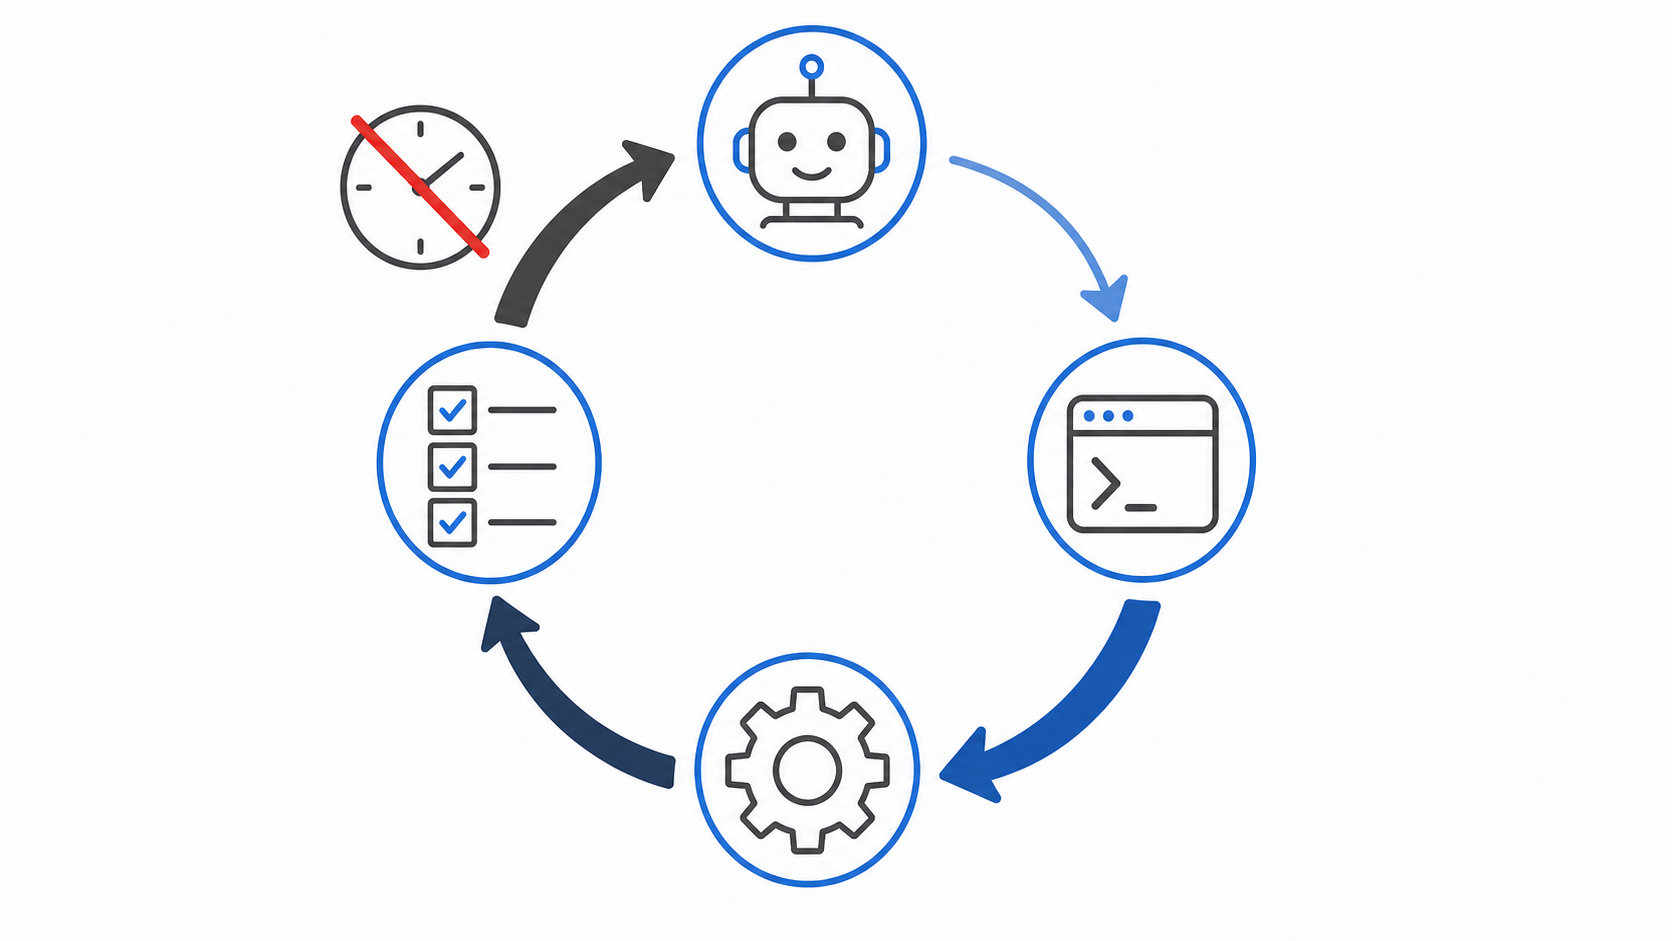
\includegraphics[width=0.72\linewidth]{figs/fig1_concept_imagegen.png}
\caption{\textbf{Loop rot.} The agent's edit--build--test loop slows with every
cycle (arrows thicken clockwise), but elapsed time never enters the agent's
observation space (struck-out clock): the loop is correctness-supervised and
time-blind.}
\label{fig:concept}
\end{figure}

We make three contributions. First, a \textbf{measurement study}
(Section~\ref{sec:measurement}): we analyze 500 verified trajectories from the
public Terminal-Bench~2.0 leaderboard --- 7 models under one harness and one
model under three harnesses --- under a five-way taxonomy of temporal waste,
and show that waste is long-tailed, kills $\sim$8\% of failed runs, and is
strongly shaped by the harness's temporal interface. Second, \textbf{\tempo{}}
(Section~\ref{sec:tempo}): a minimal, harness-level temporal-observability
layer. Third, \textbf{\textsc{RotBench}} (Section~\ref{sec:rotbench}): tasks
mined from real repositories whose maintainers historically fixed a decayed
development loop, letting us test whether time-aware agents reproduce the
refactors humans were driven to by impatience.

Our evaluation deliberately holds correctness fixed: we report unchanged
pass@1 alongside left-shifted time-to-success distributions, avoiding the
known unreliability of raw-speedup scores~\citep{todo-perfopt}.

\section{Related Work}
\label{sec:related}

\todo{Agent harness observability (component/experience/decision pillars) ---
cite AHE; position temporal observability as the fourth pillar. Terminal-Bench
/ Harbor; SWE-bench family. Context rot as the sibling phenomenon in the
context dimension. Performance-optimization benchmarks (PERFOPT-Bench) and why
raw speedup is an unreliable single-dimension score. Reflexion/self-feedback
lines: feedback signals exist for correctness, not cost.}

\section{A Measurement Study of Temporal Waste}
\label{sec:measurement}

\subsection{Data and method}

We analyze the official Terminal-Bench~2.0 leaderboard artifact repository,
which publishes each verified submission's raw Harbor job directories,
including a per-trial \texttt{trajectory.json} with microsecond ISO timestamps
per step, tool calls (including Terminus-declared wait durations), terminal
observations, and per-step token counts. We sample 500 trials: 50 each from 10
submissions --- Terminus~2 paired with 7 models (Claude Opus 4.6, GPT-5.3-Codex,
GLM-4.7, GLM-5, DeepSeek-V3.2, Kimi-k2.5, Minimax-m2.5), plus GLM-4.7 under
Claude Code and Gemini~3-Flash/3.1-Pro under Gemini CLI --- covering all 89
tasks. Consecutive step timestamps give per-step cost (execution wait plus
generation latency of the following step).

Each trial is scored by an LLM analyst agent against a five-way taxonomy:
\textbf{W1} repeat-slow (a $>$30\,s command re-run in near-identical form when
a narrower variant existed), \textbf{W2} over-wait (declared wait far exceeds
the command's need; the harness sleeps the full declaration), \textbf{W3}
under-wait churn (empty-keystroke ``wait longer'' steps, each costing a model
round-trip), \textbf{W4} same-error retry, and \textbf{W5} redundant
environment setup. Analysts are instructed to be conservative and to cite step
ids for every claim. \todo{Phase-2 adversarial verification of top exhibits;
report survival rate and inter-judge agreement.}

\subsection{Findings}

\begin{table}[t]
\centering
\small
\begin{tabular}{llrrrr}
\toprule
Harness & Model & pass & waste med. & waste p90 & failed-trial med. \\
\midrule
Terminus 2 & Claude Opus 4.6 & 66\% & 8.2\% & 38.2\% & 5.6\% \\
Terminus 2 & GPT-5.3-Codex   & 64\% & 4.3\% & 34.3\% & 2.2\% \\
Terminus 2 & Minimax-m2.5    & 45\% & 8.6\% & 30.9\% & 8.6\% \\
Terminus 2 & Kimi-k2.5       & 43\% & 10.5\% & 37.6\% & \textbf{15.7\%} \\
Terminus 2 & GLM-5           & 43\% & 6.7\% & 42.4\% & \textbf{13.9\%} \\
Terminus 2 & DeepSeek-V3.2   & 43\% & 2.8\% & 19.2\% & 3.0\% \\
Terminus 2 & GLM-4.7         & 32\% & 7.2\% & 32.4\% & 8.7\% \\
\midrule
Claude Code & GLM-4.7        & 36\% & \textbf{0.1\%} & 17.1\% & 0.2\% \\
Gemini CLI & Gemini 3-Flash  & 64\% & 0.0\% & 38.5\% & 0.0\% \\
Gemini CLI & Gemini 3.1-Pro  & 68\% & 0.0\% & \textbf{60.4\%} & 0.0\% \\
\bottomrule
\end{tabular}
\caption{Temporal waste across 436 parsed trials (500 sampled). Waste
fractions are wall-clock shares attributed to W1--W5. W2/W3 exist only in
declared-duration harnesses; cross-harness rows are comparable on W1/W4/W5
only.}
\label{tab:main}
\end{table}

\textbf{Waste is long-tailed and lethal.} Median waste is 3.7\% of wall-clock
but the 90th percentile is 34\%; 18 trials (4.1\%, or $\sim$8\% of all
failures) are \emph{time deaths}: the trial failed at or near its budget with
more than 40\% of wall-clock in W1--W5. Failed trials waste more than solved
ones (median 4.3\% vs.\ 2.7\%).

\textbf{The harness's temporal interface shapes waste.} Holding the model
fixed (GLM-4.7), moving from Terminus~2's declared-duration interface to
Claude Code's native tool calling drops median waste from 7.2\% to 0.1\%:
most of the median is mechanically manufactured by forcing blind duration
guesses. The tail, however, is harness-independent --- Gemini CLI's median is
0\% yet its p90 reaches 60\%, and it contributes 5 of the 18 time deaths,
driven by semantic waste (W1/W5) that no interface fix removes.

\textbf{Weak models die of time mismanagement.} Within Terminus~2,
failed-trial waste medians separate sharply: 2.2--5.6\% for the strongest
models (GPT-5.3-Codex, Opus 4.6) versus 13.9--15.7\% for Kimi-k2.5 and GLM-5
(the latter alone accounts for 5 time deaths). Strong models fail on hard
problems; weaker models fail on the clock.

\textbf{Some tasks are time black holes.} \texttt{fix-ocaml-gc} and
\texttt{build-pov-ray} produce $>$25\% waste in multiple independent trials
across agents, suggesting task-level structure (long compiles, slow feedback
loops) that systematically induces waste --- exactly the structure
\textsc{RotBench} isolates.

\section{\tempo{}: Making Iteration Cost Observable}
\label{sec:tempo}

\todo{Design: harness-level layer that (a) stamps every tool result with
elapsed wall-clock, (b) surfaces cumulative budget consumed / remaining, (c)
tracks per-command-template running cost and flags regressions ("this test
suite has slowed 3x since first run"). Zero model changes; in-context only.
Ablations: (a) alone vs (a)+(b) vs full. Implementation over Harbor so all
TB agents inherit it.}

\section{\textsc{RotBench}: Growth-Driven Developability Decay}
\label{sec:rotbench}

\todo{Mining pipeline (searcher/verifier/curator over GitHub history);
inclusion criteria (permissive license, structural fix commit, growth-driven
slowdown, containerized build $<$25 min, measured pre/post $>$30\%); task
card format: pre-fix snapshot + feature requests, historical fix as
reference. Report mining yield per ecosystem.}

\section{Experiments}
\label{sec:experiments}

\todo{Main claim: pass@1 unchanged, time-to-success distribution shifts left,
within-budget success rises. Baselines: Terminus 2 and one native-tool-calling
harness, each with/without \tempo{}, 3+ models. Metrics: time-to-success CDF,
within-budget success at 0.5x/1x budget, waste\_frac re-measured under \tempo{},
TIME-DEATH count. RotBench: does the agent initiate loop-restoring refactors
with/without temporal signals?}

\section{Limitations and Ethics}
\todo{LLM-judged waste labels (mitigated by adversarial verification);
leaderboard trajectories are observational, not interventional; W2/W3
harness-specificity; single-benchmark scope until RotBench results land.}

\bibliographystyle{plainnat}
\bibliography{refs}
\end{document}
